% auto-generated by scripts/gen-tables.mjs — throughput vs application-side CPU, deep fetch on PostgreSQL
\begin{figure}[htbp]
  \centering
  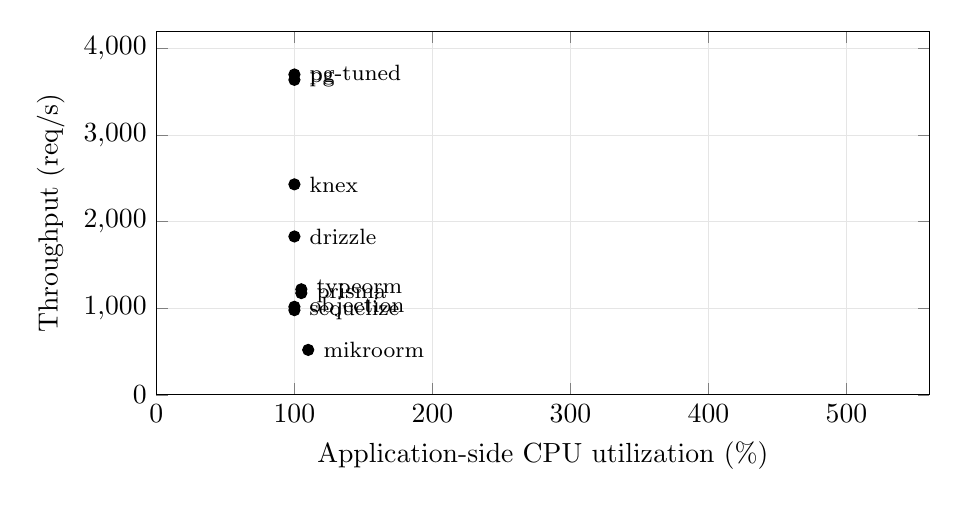
\begin{tikzpicture}
    \begin{axis}[
      width=0.94\linewidth, height=6.2cm,
      xlabel={Application-side CPU utilization (\%)}, ylabel={Throughput (req/s)},
      xmin=0, xmax=560, ymin=0, ymax=4200, xtick={0,100,200,300,400,500},
      grid=major, grid style={gray!20},
      nodes near coords, point meta=explicit symbolic,
      every node near coord/.append style={anchor=west, xshift=2pt, font=\footnotesize},
    ]
      \addplot[scatter, only marks, mark=*, scatter src=explicit symbolic] coordinates {(100,3638) [pg] (100,3700) [pg-tuned] (100,2431) [knex] (100,1829) [drizzle] (105,1175) [prisma] (100,978) [sequelize] (105,1219) [typeorm] (100,1017) [objection] (110,519) [mikroorm]};
    \end{axis}
  \end{tikzpicture}
  \caption{Throughput versus application-side CPU on the deep fetch (PostgreSQL, ten-connection pool, medians of 25 replicates). Every layer sits at about $100$--$110\%$ of one application core; the native driver leads on the throughput axis, and the slower ORMs are low on throughput at the same CPU. CPU is the server process only; database-side CPU is excluded for all layers alike.}
  \label{fig:cpu_tradeoff}
\end{figure}
